\documentclass[a4paper]{article}
\usepackage[fontsize=12pt]{scrextend}

\usepackage{tikz}
\usetikzlibrary{positioning,arrows.meta,shapes.geometric}

% --- Настройка шрифтов и локализации для XeLaTeX ---
\usepackage{fontspec}
\usepackage{xunicode}
\usepackage{xltxtra}
\usepackage{polyglossia}
\setmainlanguage{russian}
\setotherlanguage{english}
\defaultfontfeatures{Ligatures=TeX}
\setmainfont{Times New Roman}
\newfontfamily\cyrillicfont{Times New Roman}
\setmonofont{Courier New}
\newfontfamily\cyrillicfonttt{Courier New}

% --- Параметры страницы по ГОСТ 7.32-2017 (левое 30 мм, правое 10 мм, верхнее и нижнее по 20 мм) ---
\usepackage[left=30mm, right=10mm, top=20mm, bottom=20mm]{geometry}

% --- Интервалы и абзацный отступ (1.25 см, 1.5 интервал, выравнивание по ширине) ---
\usepackage{indentfirst}
\setlength{\parindent}{1.25cm}
\usepackage{setspace}
\onehalfspacing

% --- Пакеты для таблиц, списков и графики ---
\usepackage{tabularx}
\usepackage{booktabs}
\usepackage{array}
\usepackage{enumitem}
\setlist{nosep, leftmargin=\parindent}
\usepackage{graphicx}

% --- Листинги кода с подсветкой синтаксиса ---
\usepackage{listings}
\usepackage{xcolor}

\lstset{
    basicstyle=\ttfamily\footnotesize,
    columns=flexible,
    keepspaces=true,
    breaklines=true,
    frame=single,
    tabsize=2,
    showstringspaces=false,
    keywordstyle=\bfseries\color{blue!70!black},
    commentstyle=\itshape\color{green!50!black},
    stringstyle=\color{red!60!black},
    numbers=none
}

% --- Оформление заголовков разделов и подразделов по ГОСТ 7.32-2017 ---
\usepackage{titlesec}

\titleformat{\section}[block]
  {\normalfont\bfseries\filright}
  {\hspace{1.25cm}\thesection\quad}
  {0pt}
  {}

\titleformat{\subsection}[block]
  {\normalfont\bfseries\filright}
  {\hspace{1.25cm}\thesubsection\quad}
  {0pt}
  {}

\titleformat{\subsubsection}[block]
  {\normalfont\bfseries\filright}
  {\hspace{1.25cm}\thesubsubsection\quad}
  {0pt}
  {}

\titlespacing*{\section}{0pt}{18pt}{12pt}
\titlespacing*{\subsection}{0pt}{12pt}{6pt}
\titlespacing*{\subsubsection}{0pt}{10pt}{4pt}

% --- Настройка подписей к рисункам и таблицам ---
\usepackage[tableposition=top,figureposition=bottom]{caption}
\DeclareCaptionLabelSeparator{emdash}{~---~}
\captionsetup[figure]{
  name={Рисунок},
  labelsep=emdash,
  font={normalsize},
  justification=centering,
  singlelinecheck=true
}
\captionsetup[table]{
  name={Таблица},
  labelsep=emdash,
  font={normalsize},
  justification=raggedright,
  singlelinecheck=false,
  margin=0pt
}

% --- Оглавление по ГОСТ ---
\usepackage{tocloft}
\renewcommand{\cftsecleader}{\cftdotfill{\cftdotsep}}
\makeatletter
\renewcommand{\@cftmaketoctitle}{}
\makeatother

\begin{document}

% =========================================================================
% ТИТУЛЬНЫЙ ЛИСТ
% =========================================================================
\begin{titlepage}
  \singlespacing
  \centering
  {\small МИНИСТЕРСТВО НАУКИ И ВЫСШЕГО ОБРАЗОВАНИЯ РОССИЙСКОЙ ФЕДЕРАЦИИ}\\
  {\scriptsize \textbf{ФЕДЕРАЛЬНОЕ ГОСУДАРСТВЕННОЕ АВТОНОМНОЕ ОБРАЗОВАТЕЛЬНОЕ УЧРЕЖДЕНИЕ ВЫСШЕГО ОБРАЗОВАНИЯ}}\\
  {\bfseries «НАЦИОНАЛЬНЫЙ ИССЛЕДОВАТЕЛЬСКИЙ УНИВЕРСИТЕТ ИТМО»}\\[0.8cm]

  \textbf{Факультет безопасности информационных технологий}\\[0.6cm]

  \textbf{Направление подготовки: 10.03.01 Информационная безопасность} \\
  \textbf{Образовательная программа: «Технологии защиты информации»} \\[0.6cm]

  \textbf{Дисциплина:} \\
  \textit{\textbf{«Технологии и методы программирования»}} \\ [1.2cm]

  {\bfseries ОТЧЕТ ПО ЛАБОРАТОРНОЙ РАБОТЕ №4}\\
  \textit{{\bfseries «Исследование и реверс-инжиниринг алгоритмов парольной защиты исполняемых файлов методами статического анализа»}}\\[2.5cm]

  \begin{flushright}
    \textbf{Выполнил студент:} \\ [0.5em]
    Пахомов Владимир Юрьевич / \raisebox{-0.3\height}{
\includegraphics[width=1.3cm]{sign1.png}} \\
    {\scriptsize{\textit{ФИО \hspace{2cm} Подпись \hspace{0.3cm}}}} \\ [0.3cm]

    \textbf{Проверил:}\\ [0.5em]
    Ищенко Алексей Петрович / \underline{\hspace{2.5cm}} \\
    {\scriptsize{\textit{ФИО \hspace{2.5cm} Подпись \hspace{0.5cm}}}} \\ [1.2cm]

    {\scriptsize \underline{\hspace{4cm}}} \\
    {\scriptsize \textit{Отметка о выполнении}} \\
    {\scriptsize \underline{\hspace{4cm}}} \\
    {\scriptsize \textit{Дата}}
  \end{flushright}

  \vfill
  Санкт-Петербург\\
  2026
\end{titlepage}

% =========================================================================
% СОДЕРЖАНИЕ
% =========================================================================
\newpage
\pagestyle{plain}
\setcounter{page}{2}

\begin{center}
  {\bfseries СОДЕРЖАНИЕ}
\end{center}
\vspace{12pt}

\tableofcontents

% =========================================================================
% ВВЕДЕНИЕ
% =========================================================================
\newpage
\begin{center}
  {\bfseries ВВЕДЕНИЕ}
\end{center}
\addcontentsline{toc}{section}{ВВЕДЕНИЕ}

\textbf{Цель работы}: приобретение практических навыков исследования скомпилированных исполняемых модулей архитектуры x86 с использованием инструментария статического анализа, изучение низкоуровневой структуры оконных интерфейсов VCL, декомпиляция проприетарного алгоритма проверки пароля и аналитическое восстановление секретного значения без применения атак полного перебора и бинарной модификации исполняемого кода.

\textbf{Постановка задачи}:
\begin{enumerate}
  \item Провести первичный анализ исполняемого файла формата PE32 с помощью утилит статической разведки (Detect It Easy) для определения компилятора и характеристик среды сборки.
  \item Исследовать графический интерфейс приложения, зафиксировать значение открытого параметра («соли») и проанализировать логику блокировки при превышении лимита попыток ввода пароля.
  \item Извлечь и структурировать ресурсы графических форм с помощью утилиты Resource Hacker с целью выявления идентификаторов элементов управления и сигнатур обработчиков событий.
  \item В среде дизассемблера IDA Pro локализовать процедуры \texttt{FormShow} и \texttt{Button1Click}, выполнить их декомпиляцию в псевдокод и восстановить алгоритм валидации пароля.
  \item Локализовать в сегменте данных программы эталонное значение, используемое для финального сравнения с результатом обработки пользовательского ввода.
  \item Построить математическую модель обратного криптографического преобразования, выполнить посимвольный расчёт искомого пароля и осуществить практическую проверку корректности авторизации в приложении.
\end{enumerate}

% =========================================================================
% 1. АРХИТЕКТУРНЫЙ И СТРУКТУРНЫЙ АНАЛИЗ ИСПОЛНЯЕМОГО ФАЙЛА
% =========================================================================
\newpage
\section{АРХИТЕКТУРНЫЙ И СТРУКТУРНЫЙ АНАЛИЗ ИСПОЛНЯЕМОГО ФАЙЛА}

\subsection{Первичная идентификация файла и среды сборки}
На начальном этапе исследования был выполнен анализ структуры целевого исполняемого файла формата PE32. С помощью специализированной утилиты анализа бинарных файлов Detect It Easy были определены базовые характеристики исполняемого модуля (Рисунок~\ref{fig:die_window}).

\begin{figure}[!ht]
  \centering
  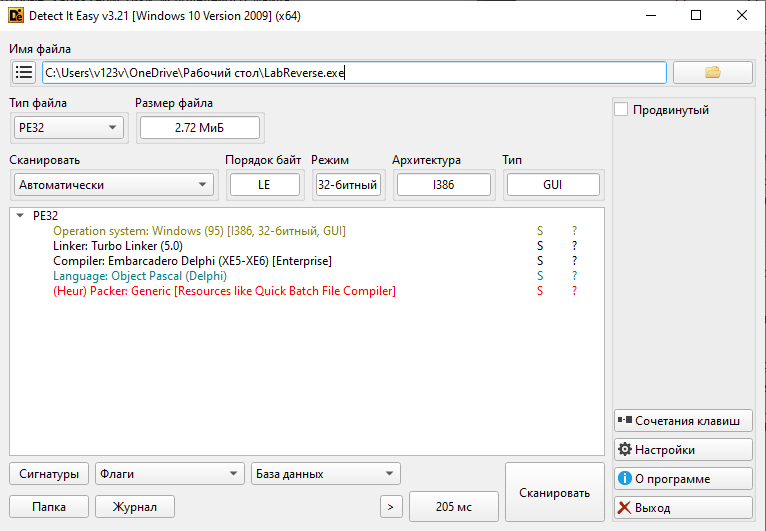
\includegraphics[width=0.75\textwidth]{img1.png}
  \caption{Результаты анализа исполняемого файла в Detect It Easy}
  \label{fig:die_window}
\end{figure}

По результатам анализа установлено, что исследуемый файл представляет собой 32-разрядное приложение Windows (PE32), собранное компилятором Embarcadero C++ Builder.

\subsection{Интерфейс пользователя и логика блокировки подбора}
При штатном запуске программа инициализирует графический интерфейс (Рисунок~\ref{fig:app_window}), содержащий следующие элементы:
\begin{itemize}
  \item Текстовое поле с индивидуально сгенерированным параметром «Секрет» (соль): \texttt{zj9b758v};
  \item Поле для ввода парольной фразы;
  \item Кнопки управления «OK» (инициация процедуры проверки) и «Выход».
\end{itemize}

\begin{figure}[h!]
  \centering
  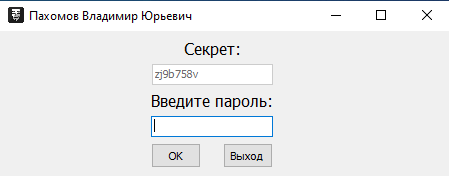
\includegraphics[width=0.65\textwidth]{img2.png}
  \caption{Графический интерфейс исследуемого приложения}
  \label{fig:app_window}
\end{figure}

В случае ввода некорректного значения программа информирует пользователя диалоговым окном «Неверный пароль!». При превышении лимита попыток ввода (более двух неудачных попыток подряд) приложение переходит в состояние блокировки длительностью 10 секунд (Рисунок~\ref{fig:wrong_and_blocked}). Данный механизм исключает практическую возможность применения методов полного перебора (brute-force).

\begin{figure}[h!]
  \centering
  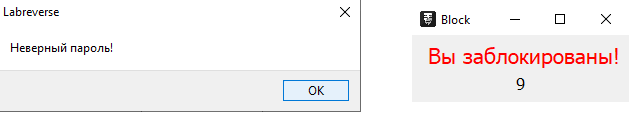
\includegraphics[width=0.8\textwidth]{img3.png}
  \caption{Окна предупреждения об ошибке и временной блокировки ввода}
  \label{fig:wrong_and_blocked}
\end{figure}

\subsection{Анализ ресурсов форм в Resource Hacker}
С целью определения внутренней структуры оконных объектов и точек привязки событий был произведен разбор секции ресурсов \texttt{RCData} с помощью утилиты Resource Hacker. В результате анализа была извлечена декларация используемых форм:

\begin{lstlisting}
object Form1: TForm1
  OnShow = FormShow
  object Label1: TLabel
    Caption = 'Введите пароль:'
  end
  object Label2: TLabel
    Caption = 'Секрет:'
  end
  object Edit1: TEdit            // поле ввода пароля
  end
  object Button1: TButton
    Caption = 'OK'
    OnClick = Button1Click       // обработчик проверки пароля
  end
  object Edit2: TEdit            // поле отображения соли
    Enabled = False
  end
end

object Form2: TForm2             // форма успешной аутентификации
  Caption = 'Form2'
  object Label1: TLabel
    Caption = 'Поздравляем, вы подобрали пароль!'
  end
end

object Form3: TForm3             // форма блокировки при переборе
  Caption = 'Block'
  OnCloseQuery = FormCloseQuery
  OnShow = FormShow
  object Label1: TLabel
    Caption = 'Вы заблокированы!'
  end
  object Timer1: TTimer
  object Timer2: TTimer
end
\end{lstlisting}

Полученное описание позволяет точно сопоставить элементы пользовательского интерфейса с обработчиками событий в бинарном коде: процедура \texttt{FormShow} отвечает за подготовку формы и отображение соли, а \texttt{Button1Click} реализует проверку введенных данных.

% =========================================================================
% 2. СТАТИЧЕСКИЙ АНАЛИЗ И ДЕКОМПИЛЯЦИЯ АЛГОРИТМА ВАЛИДАЦИИ
% =========================================================================
\newpage
\section{СТАТИЧЕСКИЙ АНАЛИЗ И ДЕКОМПИЛЯЦИЯ АЛГОРИТМА ВАЛИДАЦИИ}

\subsection{Локализация процедур обработки событий в IDA Pro}
На основе имен методов в дизассемблере IDA Pro был выполнен поиск строковых ссылок в таблице методов формы. По адресу \texttt{0x0065DC8D} в секции данных \texttt{.data} располагаются дескрипторы соответствующих процедур:

\begin{lstlisting}[language={[x86masm]Assembler}]
.data:0065DC88                 db    0
.data:0065DC89                 dd offset sub_40330C
.data:0065DC8D aButton1click   db 12,'Button1Click'
.data:0065DC9A                 db  0Fh
.data:0065DC9B                 db    0
.data:0065DC9C                 dd offset sub_404400
.data:0065DCA0 aFormshow       db 8,'FormShow',0
\end{lstlisting}

Таким образом, установлены прямые адреса подпрограмм:
\begin{itemize}
  \item \texttt{sub\_40330C} --- реализация обработчика нажатия кнопки проверки (\texttt{Button1Click});
  \item \texttt{sub\_404400} --- подпрограмма инициализации окна и соли (\texttt{FormShow}).
\end{itemize}

\subsection{Декомпиляция и исследование алгоритма Button1Click}
Декомпиляция функции \texttt{sub\_40330C} во внутреннее C-подобное представление выявила следующую логику работы алгоритма проверки:

\begin{lstlisting}[language=C]
void __fastcall sub_40330C(int a1)
{
  // Проверка соответствия длины пароля: ровно 8 символов
  v40 = sub_4042D4(v103) != 8;
  if ( v40 ) {
    // Вывод сообщения о некорректной длине строки
  } else {
    for ( j = 1; j < 9; ++j )  // Цикл по 8 символам пароля (1..8)
    {
      // Извлечение символа пароля и вычитание 48 (код '0')
      v53 = *(unsigned __int16 *)sub_404308((System::UnicodeString *)v94, j);
      v54 = v53 - 48;

      // Извлечение соответствующего символа соли и вычитание 48
      v48 = *(unsigned __int16 *)sub_404308((System::UnicodeString *)v86, j);
      v49 = v48 - 48;

      // Побитовое исключающее ИЛИ (XOR) нормализованных значений
      v42 = sub_4244FC(*v36) + v34;  // Результирующий байт XOR

      // Конвертация кода в символ через sub_4043BC и добавление в строку
      sub_4043BC(v66, v42);
      System::UnicodeString::operator+(v37, &unk_65D220, v66);
      sub_65B524(&unk_65D220, v65);
    }

    // Сравнение результирующей строки с эталоном unk_66963C
    if ( (unsigned __int8)sub_65B5C0(&unk_65D220, &unk_66963C) )
    {
      // Успешная валидация: отображение Form2
    }
    else
    {
      // Ошибка: инкремент счетчика неудачных попыток
      if ( ++dword_65D228 > 2 )
      {
        dword_65D228 = 0;
        // Запись состояния блокировки в системный реестр Windows
        System::Win::Registry::TRegistry::WriteString(v41, *v39);
        Vcl::Forms::TCustomForm::Show(*(Vcl::Forms::TCustomForm **)off_668E58); // Form3
      }
    }
  }
}
\end{lstlisting}

Анализ подпрограммы \texttt{sub\_4043BC} показал, что она выполняет форматирование через \texttt{sprintf("\%c", v42)}, то есть преобразует вычисленный числовой код в одиночный символ \texttt{Chr(v42)}.

Следовательно, для каждой позиции $i \in [0, 7]$ алгоритм выполняет элементарное математическое действие:
\[
  p_i = ord(password[i]) - 48, \quad s_i = ord(salt[i]) - 48, \quad t_i = p_i \oplus s_i
\]
Полученная 8-символьная последовательность конкатенируется в накопителе \texttt{unk\_65D220} и сравнивается с глобальной эталонной константой \texttt{unk\_66963C}.

\subsection{Локализация эталонной строки сравнения unk\_66963C}
С использованием перекрестных ссылок (XREF) к адресу \texttt{unk\_66963C} была обнаружена функция инициализации \texttt{sub\_40304C}:

\begin{lstlisting}[language={[x86masm]Assembler}]
.data:0066963C unk_66963C      db    ? ; DATA XREF: sub_40304C+14A↑o
                                       ; sub_40330C:loc_40403E↑o
\end{lstlisting}

Декомпилированный фрагмент \texttt{sub\_40304C} демонстрирует последовательное копирование строк в глобальные переменные. В ячейку \texttt{unk\_66963C} заносится строковый литерал по адресу \texttt{aN5p0d0a}:

\begin{lstlisting}[language=C]
sub_65B454(v9, aN5p0d0a);     // Загрузка эталонного литерала
sub_65B524(&unk_66963C, v9);  // Сохранение в целевую константу сравнения
\end{lstlisting}

При переходе по адресу метки \texttt{aN5p0d0a} в сегменте \texttt{.data} располагаются исходные байты строки:

\begin{lstlisting}[language={[x86masm]Assembler}]
.data:0065D29C                 db    0
.data:0065D29D aN5p0d0a        db 'N:5p0D0A',0         ; DATA XREF: sub_40304C+132↑o
.data:0065D2A6 unk_65D2A6      db    6                 ; Следующая структура данных
\end{lstlisting}

Символ двоеточия \texttt{':'} является недопустимым в идентификаторах языка C/C++, вследствие чего автоматический анализатор IDA Pro опустил его при формировании имени метки (\texttt{aN5p0d0a}). Непосредственный анализ данных подтверждает, что эталон состоит ровно из 8 символов: \textbf{\texttt{N:5p0D0A}}.

% =========================================================================
% 3. МАТЕМАТИЧЕСКОЕ ВОССТАНОВЛЕНИЕ ПАРОЛЯ И ВЕРИФИКАЦИЯ
% =========================================================================
\newpage
\section{МАТЕМАТИЧЕСКОЕ ВОССТАНОВЛЕНИЕ ПАРОЛЯ И ВЕРИФИКАЦИЯ}

\subsection{Вывод формулы обратного преобразования}
На основе установленного прямого алгоритма получена аналитическая формула восстановления каждого символа пароля:
\[
  s_i = ord(salt[i]) - 48
\]
\[
  p_i = ord(target[i]) \oplus s_i
\]
\[
  password[i] = chr(p_i + 48)
\]

\subsection{Посимвольный расчёт пароля}
В качестве исходных значений используются соль \texttt{salt = "zj9b758v"} и эталонная цепочка \texttt{target = "N:5p0D0A"}. Результаты пошагового вычисления сведены в таблицу~\ref{tab:passwd_calc}.

\begin{table}[h!]
  \caption{Посимвольное восстановление пароля обратным XOR-преобразованием}
  \label{tab:passwd_calc}
  \small
  \centering
  \begin{tabular}{|c|c|c|c|c|c|c|}
    \hline
    $i$ & salt$[i]$    & $s_i = \mathrm{ord} - 48$ & target$[i]$  & $\mathrm{ord}(\mathrm{target}[i])$ & $p_i = \mathrm{target} \oplus s$ & Символ пароля ($p_i+48$)                        \\
    \hline
    0   & \texttt{'z'} & 74                        & \texttt{'N'} & 78                                 & $78 \oplus 74 = 4$               & $4 + 48 = 52 \rightarrow$ \textbf{\texttt{4}}   \\
    1   & \texttt{'j'} & 58                        & \texttt{':'} & 58                                 & $58 \oplus 58 = 0$               & $0 + 48 = 48 \rightarrow$ \textbf{\texttt{0}}   \\
    2   & \texttt{'9'} & 9                         & \texttt{'5'} & 53                                 & $53 \oplus 9 = 60$               & $60 + 48 = 108 \rightarrow$ \textbf{\texttt{l}} \\
    3   & \texttt{'b'} & 50                        & \texttt{'p'} & 112                                & $112 \oplus 50 = 66$             & $66 + 48 = 114 \rightarrow$ \textbf{\texttt{r}} \\
    4   & \texttt{'7'} & 7                         & \texttt{'0'} & 48                                 & $48 \oplus 7 = 55$               & $55 + 48 = 103 \rightarrow$ \textbf{\texttt{g}} \\
    5   & \texttt{'5'} & 5                         & \texttt{'D'} & 68                                 & $68 \oplus 5 = 65$               & $65 + 48 = 113 \rightarrow$ \textbf{\texttt{q}} \\
    6   & \texttt{'8'} & 8                         & \texttt{'0'} & 48                                 & $48 \oplus 8 = 56$               & $56 + 48 = 104 \rightarrow$ \textbf{\texttt{h}} \\
    7   & \texttt{'v'} & 70                        & \texttt{'A'} & 65                                 & $65 \oplus 70 = 7$               & $7 + 48 = 55 \rightarrow$ \textbf{\texttt{7}}   \\
    \hline
  \end{tabular}
\end{table}

Каждый вычисленный символ строго принадлежит разрешенному множеству алфавита (строчные латинские буквы и десятичные цифры). Итоговое восстановленное значение пароля:
\begin{center}
  \textbf{\Large 40lrgqh7}
\end{center}

\subsection{Практическая верификация решения}
Ввод вычисленного значения \texttt{40lrgqh7} в диалоговое окно программы привел к успешному прохождению валидации и открытию формы \texttt{Form2} с подтверждающим сообщением (Рисунок~\ref{fig:success_window}).

\begin{figure}[h!]
  \centering
  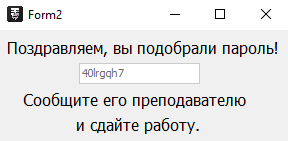
\includegraphics[width=0.55\textwidth]{img4.png}
  \caption{Успешная авторизация в программе после ввода вычисленного пароля}
  \label{fig:success_window}
\end{figure}

Программа подтвердила корректность пароля с первой попытки, что подтверждает правильность декомпилированного алгоритма и аналитических вычислений.

% =========================================================================
% ЗАКЛЮЧЕНИЕ
% =========================================================================
\newpage
\begin{center}
  {\bfseries ЗАКЛЮЧЕНИЕ}
\end{center}
\addcontentsline{toc}{section}{ЗАКЛЮЧЕНИЕ}

В процессе выполнения лабораторной работы были изучены и применены на практике методы статического реверс-инжиниринга исполняемых модулей PE32 без внесения изменений в исполняемый бинарный код.

\textbf{Основные результаты работы}:
\begin{enumerate}
  \item С помощью утилит Detect It Easy и Resource Hacker определена среда разработки исследуемого модуля, извлечена структура оконных форм и выявлены точки входа ключевых обработчиков событий (\texttt{FormShow}, \texttt{Button1Click}).
  \item В интерактивном дизассемблере IDA Pro исследована логика процедуры \texttt{sub\_40330C}, реализующей проверку фиксированной 8-символьной длины пароля и его посимвольное побитовое XOR-преобразование с параметром «соли».
  \item Локализована процедура \texttt{sub\_40304C} и извлечено истинное значение 8-байтовой эталонной строки \textbf{\texttt{N:5p0D0A}} из секции \texttt{.data}, а также объяснена причина ее сокращенного именования (\texttt{aN5p0d0a}) в базе дизассемблера.
  \item Выведена аналитическая формула обратного преобразования данных, на базе которой выполнен посимвольный расчёт искомого пароля.
  \item Получен валидный пароль \textbf{\texttt{40lrgqh7}}, полностью удовлетворяющий критериям формата (строчные латинские буквы и цифры).
  \item Выполнена успешная верификация пароля на учебном стенде без срабатывания механизмов блокировки попыток ввода.
\end{enumerate}

\end{document}